\documentclass{article}
\usepackage[a4paper,left=3cm, right=3cm, top=2cm, bottom=2cm]{geometry}
\usepackage{amsmath}
\usepackage{graphicx}
\usepackage{caption}
\usepackage{setspace}
\usepackage{xcolor}
\usepackage{titlesec}
\graphicspath{{graph/}}
\title{9.5 Linear Equations}
\date{}
\setstretch{1.2} 

% \subsection* 형식 지정 (번호 없음)
\titleformat{name=\section, numberless}
  {\normalfont\large\bfseries\color{blue}}
  {}
  {0pt}
  {}
\geometry{a4paper, margin=1in}

\begin{document}
\maketitle
This section introduces a method for solving a class of first-order differential equations that are not necessarily separable: linear differential equations. These equations are frequently encountered in various scientific applications.

\section*{Linear Differential Equations}

A first-order linear differential equation is one that can be written in the form:
\[\frac{dy}{dx} + P(x)y = Q(x)\]
where $P(x)$ and $Q(x)$ are continuous functions on a given interval. 
\\Linear equations can be solved by multiplying both sides by a suitable function called an integrating factor. The integrating factor $I(x)$ is given by:
\[I(x) = e^{\int P(x) \, dx}\]

\section*{Derivation of the Integrating Factor}
To solve $\frac{dy}{dx} + P(x)y = Q(x)$, we want to find a function $I(x)$ such that when we multiply the entire equation by $I(x)$, the left side becomes the derivative of a product, specifically $\frac{d}{dx}[I(x)y]$. Multiplying by $I(x)$ gives:
\[I(x)\frac{dy}{dx} + I(x)P(x)y = I(x)Q(x)\]
From the product rule, we know that:
\[\frac{d}{dx}[I(x)y] = I(x)\frac{dy}{dx} + I'(x)y\]
Comparing the two expressions, we must have $I(x)P(x)y = I'(x)y$, which simplifies to:
\[I'(x) = I(x)P(x)\]
This is a separable differential equation for $I(x)$. Separating variables and integrating gives:
\[\int \frac{1}{I(x)} \, dI = \int P(x) \, dx \quad \implies \quad \ln|I(x)| =\int P(x)\, dx\]
Exponentiating both sides gives the integrating factor. After multiplying the original equation by $I(x)$, we get:
\[\frac{d}{dx}[I(x)y] = I(x)Q(x)\]
Integrating both sides and solving for y yields the general solution:
\[y(x) = \frac{1}{I(x)} \left[ \int I(x)Q(x) \, dx + C \right]\]

\paragraph{To solve a linear differential equation $y'+P(x)y=Q(x)$}
\begin{enumerate}
  \item Identify $P(x)$ and $Q(x)$.
  \item Calculate the integrating factor $I(x) = e^{\int P(x) \, dx}$.
  \item Multiply both sides of the differential equation by $I(x)$.
  \item Recognize the left side as $\frac{d}{dx}[I(x)y]$.
  \item Integrate both sides with respect to x.
\end{enumerate}
\subsubsection*{Example 1: Solving a Linear Differential Equation}
Solve the differential equation $\frac{dy}{dx} + 3x^2 y = 6x^2$.

\paragraph{Solution:}
This is a linear equation with $P(x) = 3x^2$ and $Q(x) = 6x^2$. The integrating factor is:
\[I(x) = e^{\int 3x^2 \, dx} = e^{x^3}\]
Multiplying the equation by $I(x)$ and recognizing the left side as a product rule derivative gives:
\[\frac{d}{dx}(e^{x^3} y) = 6x^2 e^{x^3}\]
Integrating both sides and solving for y, we get:
\[y = 2 + Ce^{-x^3}\]


\subsubsection*{Example 2: Initial-Value Problem}
Find the solution of the initial-value problem $x^2 y' + xy = 1$, for $x>0$, with $y(1)=2$.

\paragraph{Solution:}
First, write the equation in standard form: $y' + \frac{1}{x}y = \frac{1}{x^2}$. Here, $P(x) = 1/x$ and $Q(x) = 1/x^2$. The integrating factor is:
\[I(x) = e^{\int \frac{1}{x} \, dx} = e^{\ln|x|} = x \quad (\text{since } x>0)\]
Multiplying by $x$ gives $\frac{d}{dx}(xy) = \frac{1}{x}$. Integrating both sides gives $xy = \ln x + C$.
Using the initial condition $y(1)=2$, we find $C=2$. The solution is:
\[y = \frac{\ln x + 2}{x}\]

\subsubsection*{Example 3: Solutions Involving Non-Elementary Integrals}
Solve $y' + 2xy = 1$.

\paragraph{Solution:}
With $P(x)=2x$ and $Q(x)=1$, the integrating factor is $I(x) = e^{\int 2x \, dx} = e^{x^2}$. Multiplying by $I(x)$ gives:
\[\frac{d}{dx}(e^{x^2}y) = e^{x^2}\]
Integrating both sides, we get:
\[e^{x^2}y = \int e^{x^2} \, dx + C\]
The integral $\int e^{x^2} \, dx$ cannot be expressed in terms of elementary functions, but it is a valid function. The solution is:
\[y = e^{-x^2} \int e^{x^2} \, dx + Ce^{-x^2}\]
\begin{figure}[htbp]
    \centering
    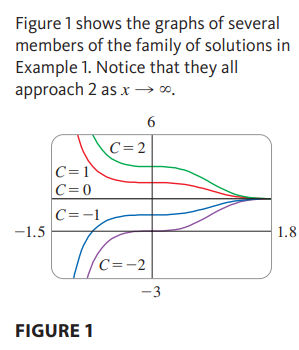
\includegraphics[width=0.3\textwidth]{graph5.png}
    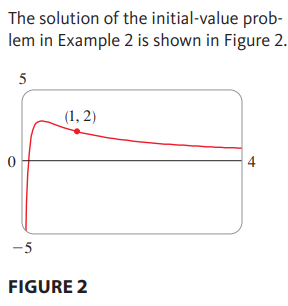
\includegraphics[width=0.3\textwidth]{graph6.png} 
    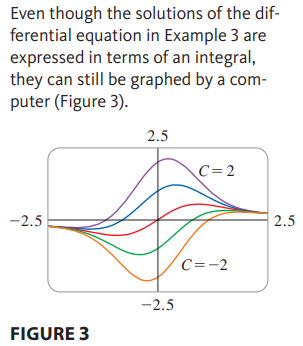
\includegraphics[width=0.3\textwidth]{graph7.png} % <-- 실제 이미지 파일명으로 변경
\end{figure}

\section*{Application to Electric Circuits}
First-order linear differential equations model the current $I(t)$ in a simple series circuit. Kirchhoff's Law gives the equation:
\[L \frac{dI}{dt} + RI = E(t)\]

\subsubsection*{Example 4: Current with a Constant Voltage}
A circuit has $R=12\Omega$, $L=4H$, a constant voltage $E(t)=60V$, and $I(0)=0$. Find $I(t)$.

\paragraph{Solution:}
The differential equation is $4 \frac{dI}{dt} + 12I = 60$, which simplifies to $\frac{dI}{dt} + 3I = 15$. The integrating factor is $e^{3t}$. The solution process yields:
\[I(t) = 5 + Ce^{-3t}\]
Using the initial condition $I(0)=0$, we find $C=-5$. The current is:
\[I(t) = 5(1 - e^{-3t})\]

\subsubsection*{Example 5: Current with a Variable Voltage}
The circuit is the same as in Example 4 ($R=12\Omega, L=4H$), but with a variable voltage $E(t)=60\sin(30t)$. Find $I(t)$ assuming $I(0)=0$.

\paragraph{Solution:}
The differential equation is $\frac{dI}{dt} + 3I = 15\sin(30t)$. The integrating factor is $e^{3t}$.
\[\frac{d}{dt}(e^{3t}I) = 15e^{3t}\sin(30t)\]
Using the integral formula $\int e^{ax}\sin(bx) \, dx = \frac{e^{ax}}{a^2+b^2}(a\sin(bx) - b\cos(bx))$, we integrate both sides:
\[e^{3t}I = 15 \left( \frac{e^{3t}}{3^2+30^2}(3\sin(30t) - 30\cos(30t)) \right) + C\]
\[e^{3t}I = \frac{5}{101}e^{3t}(\sin(30t) - 10\cos(30t)) + C\]
The general solution for the current is:
\[I(t) = \frac{5}{101}(\sin(30t) - 10\cos(30t)) + Ce^{-3t}\]
Using the initial condition $I(0)=0$:
\[0 = \frac{5}{101}(0 - 10) + C \implies C = \frac{50}{101}\]
Thus, the final solution is:
\[I(t) = \frac{5}{101}(\sin(30t) - 10\cos(30t)) + \frac{50}{101}e^{-3t}\]
\begin{figure}[htbp]
    \centering
    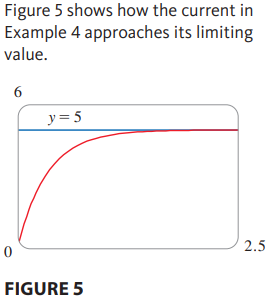
\includegraphics[width=0.3\textwidth]{graph8.png}
    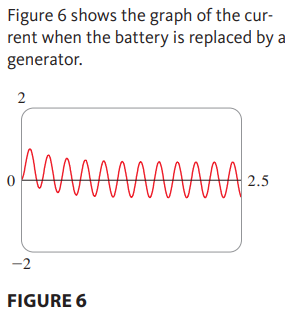
\includegraphics[width=0.3\textwidth]{graph9.png} % <-- 실제 이미지 파일명으로 변경
\end{figure}

\end{document}
